\documentclass[red]{beamer}

\usepackage[T1]{fontenc}
\usepackage[utf8]{inputenc}
\usepackage[frenchb]{babel}

\usetheme{Warsaw}

\setbeamertemplate{navigation symbols}{%
\insertslidenavigationsymbol
}


\begin{document}	
	\begin{frame}
	\frametitle{Les yeux, le cerveau et l'image}
	\framesubtitle{Schéma de l'œil}
	\begin{center}
    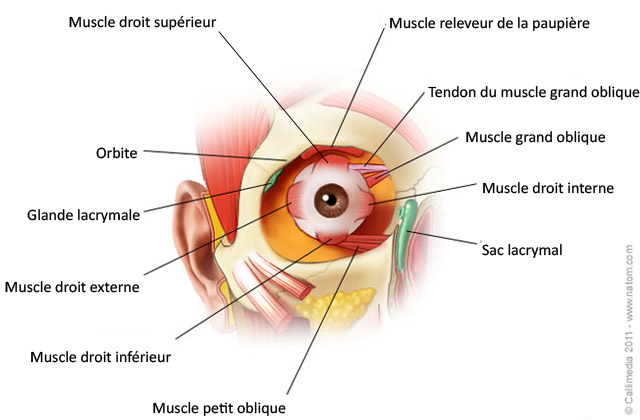
\includegraphics[scale=0.47]{oeil.jpg}
    \end{center}
	\end{frame}
	
	\begin{frame}
	\frametitle{Les yeux, le cerveau et l'image}
	\framesubtitle{Coupe de l'œil}
	\begin{center}
    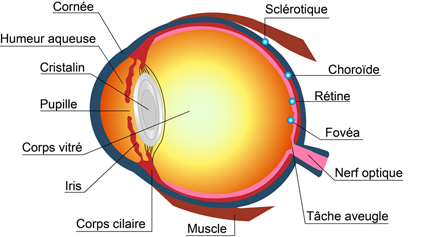
\includegraphics[scale=0.7]{schema_oeil.jpg}
    \end{center}
    \end{frame}
	
	\begin{frame}
	\frametitle{Fonctionnement de l'œil}
	\framesubtitle{Réfraction et dispersion}
		\begin{figure}
			\begin{minipage}[c]{.46\linewidth}
				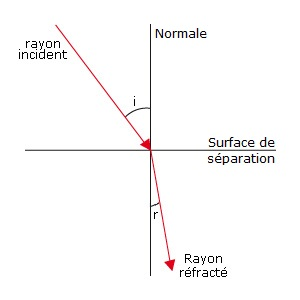
\includegraphics[scale=0.6]{refraction.jpg}
			\end{minipage} \hfill
			\begin{minipage}[c]{.46\linewidth}
		    	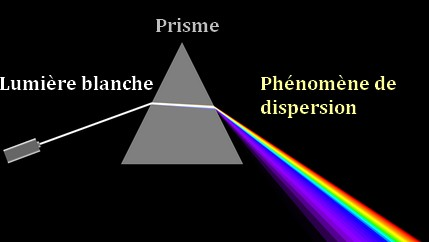
\includegraphics[scale=0.35]{dispersion.jpg} 
		    \end{minipage}
		\end{figure}
	\end{frame}	
	
	\begin{frame}
	\frametitle{Fonctionnement de l'œil}
	\framesubtitle{Lentille convergente et formation d'une image}
	\begin{figure}
		\begin{minipage}[c]{.46\linewidth}
			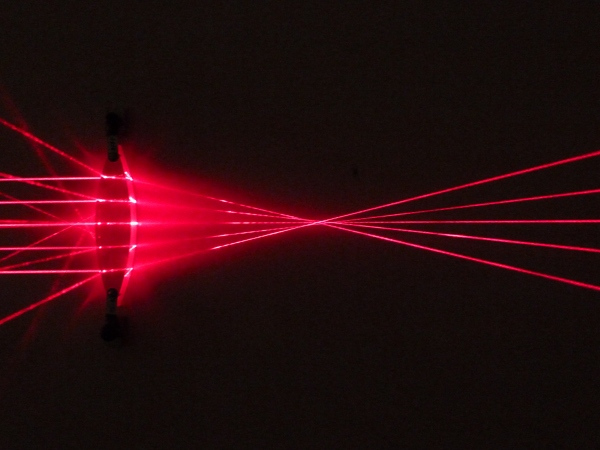
\includegraphics[scale=0.25]{lentille_convergente}
		\end{minipage} \hfill
		\begin{minipage}[c]{.46\linewidth}
	    	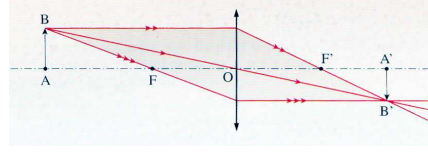
\includegraphics[scale=0.45]{formation_image} 
	    \end{minipage}
	\end{figure}
	\end{frame}
	
	\begin{frame}
	\frametitle{La lumière et l'œil}
	\framesubtitle{Les rayons lumineux}
	\begin{center}
	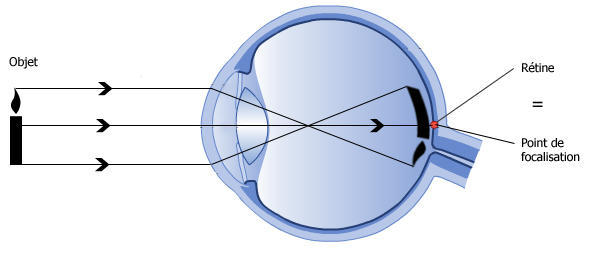
\includegraphics[scale=0.2]{rayons_lumineux.jpg}
	\end{center}
	\end{frame}
	
	\begin{frame}
	\frametitle{La rétine}
	\framesubtitle{Composition}
	\begin{center}
    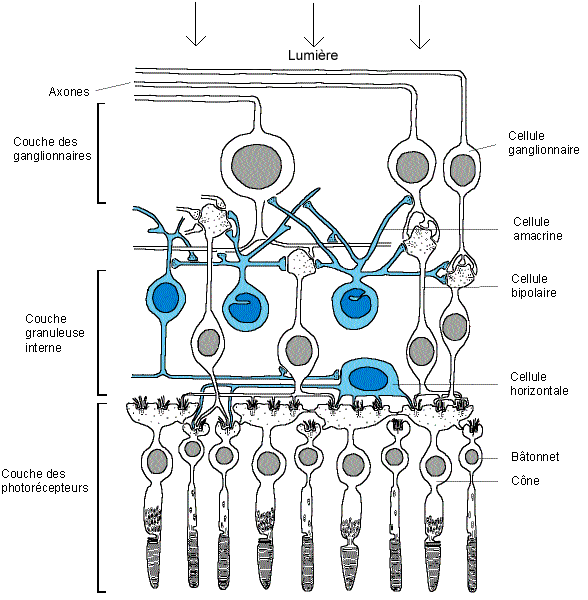
\includegraphics[scale=0.35]{retine.png}
    \end{center}
	\end{frame}
\end{document}